\documentclass[tikz, border=10pt]{standalone}
\usepackage{pgfplots}
\pgfplotsset{compat=1.18}
\usepackage{amsmath}

\begin{document}
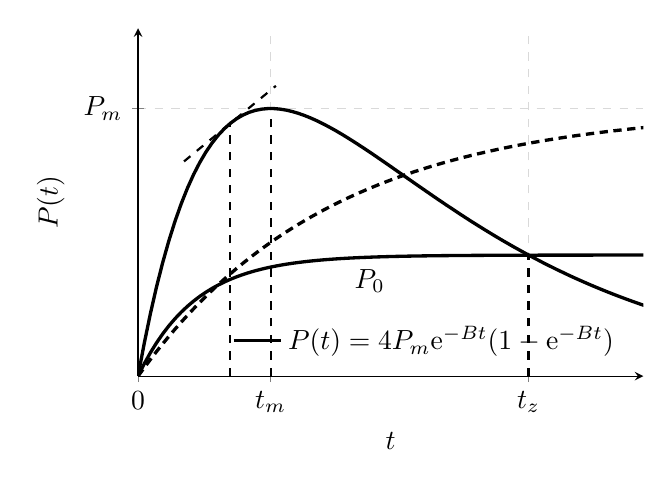
\begin{tikzpicture}
  % Parameter zentral definieren
  \pgfmathsetmacro{\Pm}{4}    % maksimumo P_m
  \pgfmathsetmacro{\B}{1.2}   % koef. B
  \pgfmathsetmacro{\C}{4}   % koef. C

  % tempo de maksiumo t_m = ln(2) / B 
  \pgfmathsetmacro{\tm}{ln(2)/\B}

  % punktoj kaj valoroj en t0 kaj tz
  \pgfmathsetmacro{\tzero}{0.4}
  \pgfmathsetmacro{\ttz}{1.7}
  \pgfmathsetmacro{\Pzero}{4 * \Pm * exp(-\B * \tzero) * (1 - exp(-\B * \tzero))}
  \pgfmathsetmacro{\Ptz}{4 * \Pm * exp(-\B * \ttz) * (1 - exp(-\B * \ttz))}

  % 2. dekliveco de la tangenot ĉe P(t_0)
  % P'(t) = 4 * Pm * B * (2 * exp(-2*B*t) - exp(-B*t))
  \pgfmathsetmacro{\slope}{4 * \Pm * \B * (2 * exp(-2 * \B * \tzero) - exp(-\B * \tzero))}

  \begin{axis}[
    width=8cm,
    height=6cm,
    axis lines=left,
    xlabel={$t$},
    ylabel={$P(t)$},
    xmin=0, xmax=2.2,
    ymin=0, ymax=5.2,    
    % aksomarkoj por 0, t_0, t_m, t_z sur X-akso
    xtick={0, \tm, \ttz},
    xticklabels={0, $t_m$, $t_z$},
    ytick={\Pm},
    yticklabels={$P_m$},
    grid=major,
    grid style={dashed, gray!30},
    samples=150,
    domain=0:4,
    legend pos=south east,
    legend style={
      fill=none,
      draw=none
    }
  ]

    % Die Funktion P(t) = 4 * P_m * exp(-B*t) * (1 - exp(-B*t))
    \addplot[black, very thick] {4 * \Pm * exp(-\B * x) * (1 - exp(-\B * x))};
    \addlegendentry{$P(t) = 4P_m \mathrm{e}^{-Bt}(1-\mathrm{e}^{-Bt})$}

    \addplot[black, dash pattern=on 3pt off 2pt, very thick] {\Pm * (1 - exp(-\B * x))};
    %\addlegendentry{$P_0(t)$}

    \addplot[black, very thick] {\Ptz * (1 - exp(-\C * x))};
    \node[above right, black] at (axis cs:0.9, 1.1) {$P_0$};

    %\addlegendentry{$P_0(t)$}

    % vertikalo ĉe la maksiumo t_m 
    \draw[black, dashed, thick] (axis cs:\tm, 0) -- (axis cs:\tm, \Pm);

    % horizontalo ĉe P_m 
    %\draw[black, dashed, thick] (axis cs:0, \Pm) -- (axis cs:\tm, \Pm);

    % punkto ĉe la maksimumo de P(t)
    %\fill[black] (axis cs:\tm, \Pm) circle (2.5pt);

    % vertikaloj en t0 kaj tz
    \draw[black, dashed, thick] (axis cs:\tzero, 0) -- (axis cs:\tzero, \Pzero);
    \draw[black, dashed, thick] (axis cs:\ttz,   0) -- (axis cs:\ttz,   \Ptz);

    % tangento ĉe t0
    \addplot[black, dashed, thick, domain=\tzero-0.2:\tzero+0.2, samples=2] {\Pzero + \slope * (x - \tzero)};

    % funkcivaloroj tie kiel punktoj
    %\fill[black] (axis cs:\tzero, \Pzero) circle (2pt);
    %\fill[black] (axis cs:\ttz,   \Ptz)   circle (2pt);

  \end{axis}
\end{tikzpicture}
\end{document}